\documentclass[11pt]{article}

% =============================================================================
% PACKAGES
% =============================================================================
\usepackage[margin=1in]{geometry}
\usepackage{amsmath,amssymb}
\usepackage{booktabs}
\usepackage{graphicx}
\usepackage[colorlinks=true,linkcolor=blue,citecolor=blue,urlcolor=blue]{hyperref}
\usepackage{caption}
\usepackage{subcaption}
\usepackage{xcolor}
\usepackage{float}
\usepackage{setspace}
\usepackage{lmodern}
\usepackage{fancyhdr}
\usepackage{titling}

% =============================================================================
% DOCUMENT SETTINGS
% =============================================================================
\setstretch{1.15}
\graphicspath{{figures/}}

% Header/Footer
\pagestyle{fancy}
\fancyhf{}
\lhead{Fixed Income Allocation Strategy}
\rhead{Regentfund Project}
\cfoot{\thepage}
\renewcommand{\headrulewidth}{0.4pt}

% =============================================================================
% TITLE PAGE
% =============================================================================
\title{%
    \vspace{-1cm}
    \textbf{Fixed Income Allocation Strategy}\\[0.5cm]
    \large\textit{A Momentum-Based Tactical Framework for the Regentfund Portfolio}
}
\author{%
    Taiya Shiva\\
    \small Hawk Center for Investment Analysis
}
\date{March 2026}

% =============================================================================
% DOCUMENT BEGIN
% =============================================================================
\begin{document}

% Title Page
\begin{titlepage}
    \centering
    \vspace*{3cm}

    {\Huge\bfseries Fixed Income Allocation Strategy\par}
    \vspace{1cm}
    {\Large\itshape A Momentum-Based Tactical Framework for the Regentfund Portfolio\par}

    \vspace{2cm}

    {\large Taiya Shiva\par}
    \vspace{0.5cm}
    {\normalsize Hawk Center for Investment Analysis\par}

    \vspace{2cm}

    {\large March 2026\par}

    \vfill

    {\small Prepared for the Regentfund Fixed Income Portfolio\par}
\end{titlepage}

% =============================================================================
% ABSTRACT
% =============================================================================
\begin{abstract}
\noindent
This paper presents a systematic tactical allocation framework for fixed income portfolios that addresses the fundamental challenge of time-varying risk premia in credit and duration markets. Traditional static allocations to investment grade corporate bonds, high yield debt, and government securities expose portfolios to regime shifts in credit cycles and rate environments simultaneously---a structural vulnerability that manifested dramatically during the 2008 financial crisis, the 2020 COVID-19 dislocation, and the 2022 rate shock.

We develop a three-layer defense mechanism comprising: (1) a cross-asset momentum filter using equity markets as an early warning system for credit deterioration, (2) trend confirmation through a blended momentum indicator calibrated to credit cycle frequencies, and (3) risk-triggered rebalancing that overrides scheduled trading when defensive positioning is required. The framework is implemented across four strategy variants accommodating different operational constraints.

Our recommended implementation---Strat 3 (Momentum), which combines daily proportional allocation with momentum-based Treasury signals---achieves a Sharpe ratio of 0.37 compared to $-0.04$ for the static benchmark, while reducing maximum drawdown by 44\% (from $-20.89\%$ to $-11.71\%$). The framework adheres to Regentfund's 12\% high yield concentration limit while delivering meaningful risk-adjusted outperformance through systematic identification of macro factor persistence rather than statistical arbitrage.
\end{abstract}

\newpage
\tableofcontents
\newpage

% =============================================================================
% SECTION 1: INTRODUCTION
% =============================================================================
\section{Introduction}

\subsection{The Fixed Income Allocation Problem}

Unlike equity markets where returns are dominated by a single systematic risk factor, fixed income returns are driven by two distinct and often conflicting systematic exposures: \textit{credit risk}---the compensation for bearing default probability---and \textit{duration risk}---the sensitivity to changes in the general level of interest rates. A portfolio holding investment grade corporate bonds, high yield debt, and government securities simultaneously bears exposure to both risk factors, creating a structural vulnerability to regime shifts that static allocation methodologies cannot address.

During credit stress events, high yield spreads can widen by 500--1000 basis points as markets reprice default expectations, transforming what appeared to be attractive carry into significant capital destruction. The 2008--2009 financial crisis saw high yield spreads exceed 2000 basis points; the March 2020 COVID-19 dislocation produced a 600 basis point widening in under three weeks. Simultaneously, rising rate environments---such as the 2022 Federal Reserve tightening cycle---inflict losses on duration-heavy allocations regardless of credit quality, as investment grade and government bond portfolios experienced their worst drawdowns in decades.

A tactical framework capable of systematically rotating exposure based on observable market signals---without relying on discretionary manager judgment---addresses a genuine structural need in institutional fixed income portfolio management. Such a framework must balance the competing demands of responsiveness to deteriorating conditions, stability to avoid excessive turnover costs, and operational feasibility within institutional trading constraints.

\subsection{Asset Universe and Benchmark}

The framework operates on three primary fixed income asset classes, each representing a distinct risk-return profile within the credit-duration spectrum:

\begin{itemize}
    \item \textbf{H5A4 (ICE BofA US High Yield Index)}: High yield corporate debt carries the widest credit spread over investment grade, compensating investors for elevated default risk. In normal conditions, this spread provides attractive carry; during credit stress, high yield exhibits equity-like drawdown characteristics as spread widening dominates coupon income.

    \item \textbf{C5A0 (ICE BofA US Investment Grade Corporate Index)}: Investment grade corporate bonds balance credit spread carry with moderate duration exposure. While less volatile than high yield during credit events, investment grade remains vulnerable to both spread widening and rate increases.

    \item \textbf{G5O2 (ICE BofA US Treasury Index)}: Government bonds serve as the flight-to-quality anchor with zero credit risk. Treasuries typically exhibit negative correlation to credit assets during risk-off episodes---a characteristic the framework explicitly leverages---but bear full duration exposure to rate regime shifts.
\end{itemize}

The benchmark portfolio reflects Regentfund's current static allocation: 66.5\% C5A0 (investment grade), 9.5\% H5A4 (high yield), 19.0\% G5O2 (government), and 5.0\% cash. This passive baseline delivered $-0.14\%$ annualized return with $-20.89\%$ maximum drawdown over the 1997--2025 sample period, illustrating the vulnerability of static allocations to the combined credit and duration shocks experienced during this period.

\subsection{Why Momentum Works in Fixed Income}

The application of momentum signals to fixed income markets requires careful theoretical grounding, as the mechanisms driving momentum in credit and duration differ fundamentally from those in equity markets.

In equity markets, momentum is often attributed to behavioral factors---investor underreaction to new information, herding behavior, and gradual diffusion of news across market participants. In fixed income markets, momentum reflects something more structural: the \textit{slow-moving nature of fundamental credit and rate dynamics}.

Credit spread cycles evolve gradually because corporate default risk changes gradually. When corporate credit conditions deteriorate, spreads widen progressively as:
\begin{enumerate}
    \item Lenders reassess default probabilities based on accumulating evidence of fundamental weakness
    \item Covenant violations and debt service coverage ratios deteriorate over multiple quarters
    \item Rating agencies---historically lagging indicators---downgrade issuers in response to realized deterioration
    \item Institutional investors with mandate constraints are forced to reduce exposure
\end{enumerate}

This gradual adjustment process---reflecting the fundamentally cash-flow-based nature of credit analysis---creates persistent directional trends in credit spread movements. A spread widening event rarely reverses within days; credit cycles operate on quarterly and annual horizons.

Similarly, interest rate regimes exhibit persistence because central bank policy operates on multi-quarter horizons. Federal Reserve tightening and easing cycles are well-telegraphed through forward guidance, dot plots, and macroeconomic projections. Rate trends persist because the underlying economic conditions driving policy decisions---inflation, employment, growth---themselves exhibit persistence.

The blended momentum framework presented here explicitly targets these fundamental frequencies. The 60--120 day lookback windows (combined 70\% weight) correspond to the typical duration of credit spread cycles, while the 240-day lookback identifies sustained rate regime shifts. This is not statistical arbitrage---it is systematic identification of macro factor persistence grounded in the structural characteristics of fixed income markets.

\subsection{Implementation Constraints}

Two binding constraints shape the final implementation:

\begin{enumerate}
    \item \textbf{12\% maximum high yield allocation}: Regentfund's portfolio guidelines limit credit concentration risk by capping H5A4 exposure at 12\% of portfolio value. This constraint reflects prudent risk management given high yield's equity-like drawdown characteristics during stress events.

    \item \textbf{Monthly rebalancing cadence}: Institutional operational requirements restrict portfolio adjustments to month-end, with the exception of risk-triggered defensive repositioning. This constraint reduces transaction costs and operational complexity but requires the framework to preserve signal value across multi-week holding periods.
\end{enumerate}

\subsection{Strategy Roadmap}

The framework produces four final strategy variants, organized as a two-by-two matrix based on the G5O2 signal methodology and rebalancing frequency:

\begin{table}[H]
\centering
\caption{Strategy Variants}
\begin{tabular}{lcc}
\toprule
& \textbf{Standard G5O2 Signal} & \textbf{Momentum G5O2 Signal} \\
\midrule
\textbf{Daily Rebalancing} & Strat 3 & Strat 3 (Momentum) \\
\textbf{Monthly Rebalancing} & Monthly Strat & Monthly Strat (Momentum) \\
\bottomrule
\end{tabular}
\end{table}

The ``standard'' G5O2 signal applies the same cross-asset momentum filter used for credit assets, while the ``momentum'' variant uses a standalone threshold-based signal optimized specifically for Treasury duration dynamics.

% =============================================================================
% SECTION 2: QUANTITATIVE FRAMEWORK
% =============================================================================
\section{Quantitative Framework}

\subsection{Blended Momentum Signal (BMOM)}

The foundation of the tactical framework is a blended momentum indicator that combines price momentum across multiple lookback horizons, weighted to emphasize frequencies corresponding to credit and rate cycle dynamics:

\begin{equation}
\text{BMOM}_i(t) = 0.15 \cdot \text{Mom}_{i,20}(t) + 0.35 \cdot \text{Mom}_{i,60}(t) + 0.35 \cdot \text{Mom}_{i,120}(t) + 0.15 \cdot \text{Mom}_{i,240}(t)
\label{eq:bmom}
\end{equation}

where $\text{Mom}_{i,n}(t)$ denotes the $n$-day price return for asset $i$ at time $t$:

\begin{equation}
\text{Mom}_{i,n}(t) = \frac{P_i(t) - P_i(t-n)}{P_i(t-n)}
\end{equation}

The weighting structure reflects fixed income market dynamics:

\begin{itemize}
    \item \textbf{60 and 120-day horizons (combined 70\% weight)}: These lookbacks correspond to the typical duration of credit spread cycles---the period from initial deterioration in corporate fundamentals to eventual repricing in secondary markets. Credit events unfold over months, not days; rating downgrades follow earnings deterioration by quarters.

    \item \textbf{240-day horizon (15\% weight)}: Identifies structural rate regime shifts driven by multi-quarter Federal Reserve policy cycles. This component ensures the framework recognizes sustained duration trends rather than tactical rate volatility.

    \item \textbf{20-day horizon (15\% weight)}: Provides tactical responsiveness to accelerating dislocations without overweighting short-term noise. This component triggers earlier exits during rapidly deteriorating conditions.
\end{itemize}

\begin{figure}[H]
    \centering
    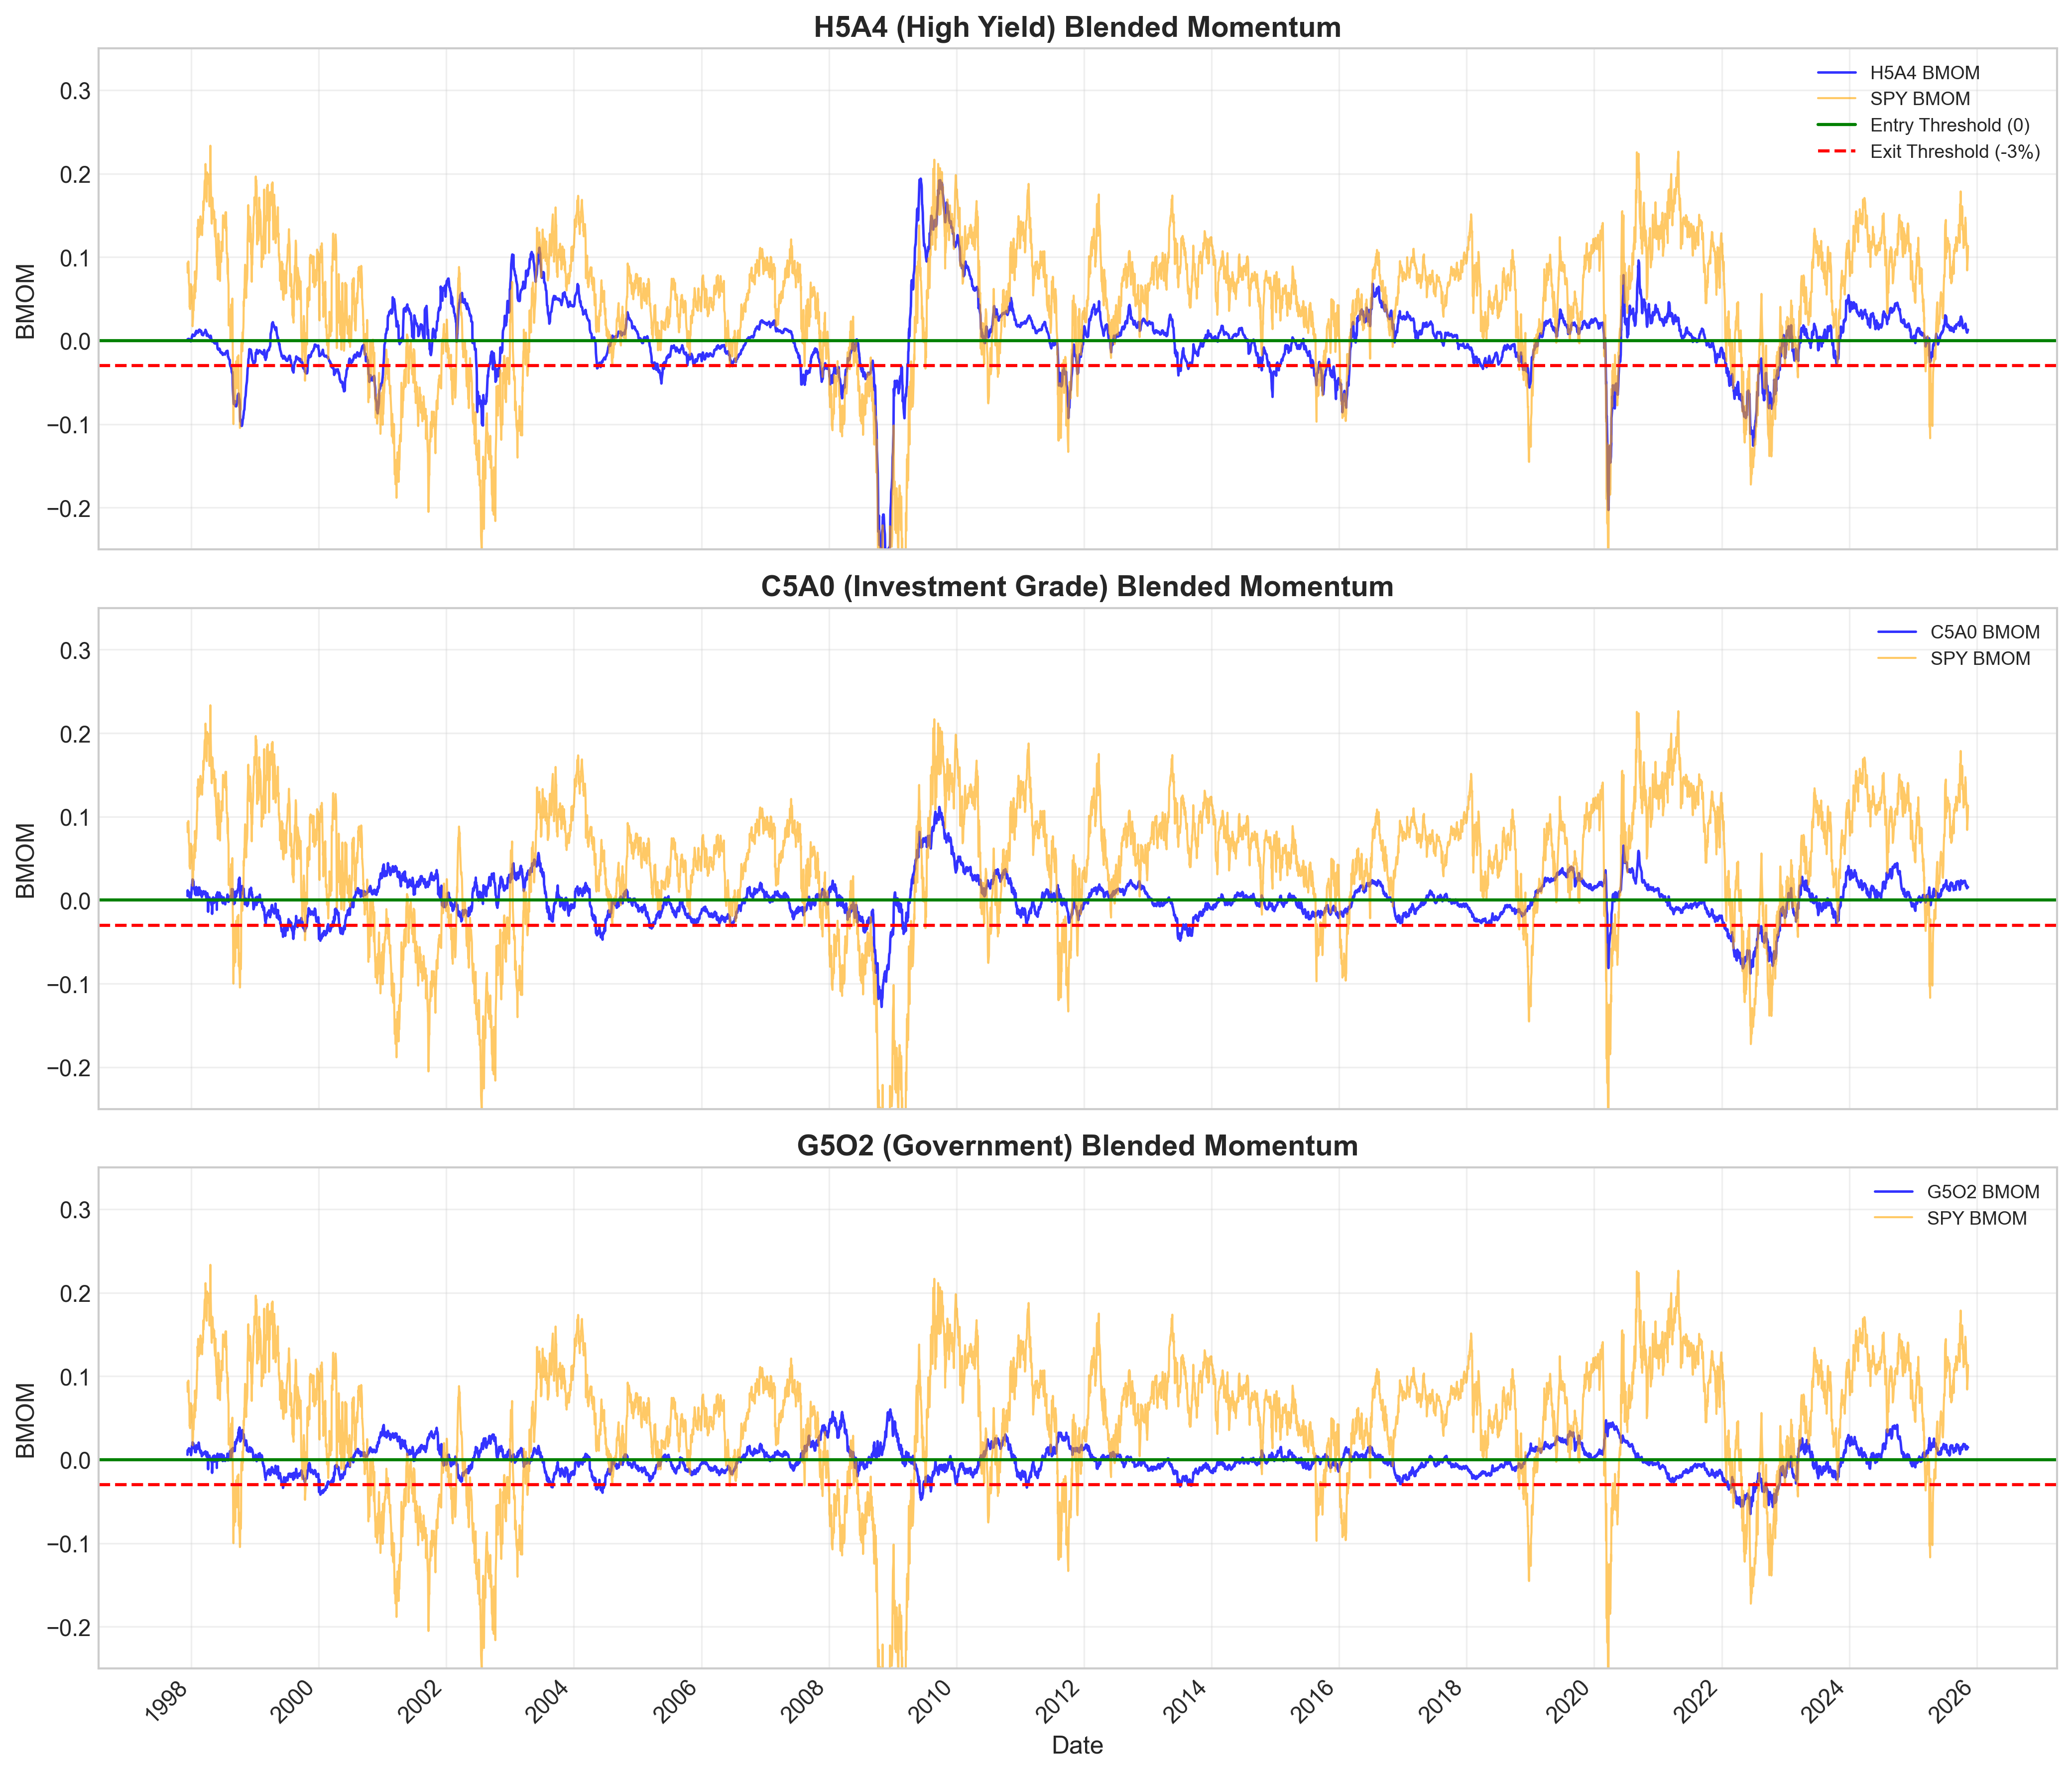
\includegraphics[width=\textwidth]{fig_bmom_signals.png}
    \caption{BMOM indicators for H5A4, C5A0, and G5O2 with SPY benchmark overlay. Entry threshold at 0 (solid green line), exit threshold at $-3\%$ (dashed red). The simultaneous deterioration of fixed income and equity BMOM during 2008, 2020, and 2022 confirms the cross-asset filtering rationale.}
    \label{fig:bmom}
\end{figure}

Figure~\ref{fig:bmom} displays the BMOM indicators for each fixed income asset class alongside the SPY (equity market) BMOM. The largest credit drawdown events---2008 financial crisis, 2020 COVID-19, and 2022 rate shock---are clearly visible as simultaneous multi-standard-deviation drops across both fixed income and equity BMOM series, validating the cross-asset dual-weakness filter discussed in the following section.

\subsection{Signal Generation: Cross-Asset Momentum Filter}

The binary signal generation mechanism leverages the equity-credit lead-lag relationship. For each asset $i$, define the exit conditions:

\begin{align}
C_1: \quad & \text{BMOM}_{\text{SPY}}(t-1) > -0.03 \wedge \text{BMOM}_{\text{SPY}}(t) < -0.03 \wedge \text{BMOM}_i(t) < -0.03 \\
C_2: \quad & \text{BMOM}_i(t-1) > -0.03 \wedge \text{BMOM}_i(t) < -0.03 \wedge \text{BMOM}_{\text{SPY}}(t) < -0.03
\end{align}

The signal logic is then:

\begin{equation}
\text{Signal}_i(t) = \begin{cases}
0 & \text{if } (C_1 \vee C_2) \wedge \text{Mom}_{i,240}(t) < 0 \quad \text{(Exit)} \\
1 & \text{if } \text{BMOM}_i(t) > 0 \quad \text{(Entry)} \\
\text{Signal}_i(t-1) & \text{otherwise} \quad \text{(Hold)}
\end{cases}
\end{equation}

The rationale for using SPY (the S\&P 500) as the benchmark filter stems from market microstructure: equity markets are highly liquid with continuous price discovery, immediately incorporating macro deterioration into valuations. Corporate bond markets---particularly high yield---feature lower liquidity, over-the-counter trading structures, and institutional holding patterns that delay price adjustment. Equity BMOM weakness therefore \textit{leads} credit spread widening by days to weeks, providing an early warning mechanism grounded in the equity-credit lead-lag relationship.

The 240-day trend confirmation ($\text{Mom}_{240} < 0$) prevents exits during temporary credit pullbacks within fundamentally sound rate environments. This filter ensures the framework responds to genuine regime shifts rather than volatility within stable trends.

For G5O2 (Treasuries), the dual-weakness logic serves a different purpose. Treasuries typically \textit{benefit} from equity weakness through flight-to-quality flows. The cross-below filter for G5O2 specifically identifies the rare but dangerous regime of simultaneous equity and Treasury weakness---stagflationary or broad deleveraging environments where even safe-haven assets sell off (e.g., 2022 rate shock, 2013 taper tantrum).

\subsection{Drawdown Differential Override (Strategy 2 Layer)}

The base signal logic can produce premature exits during market dislocations where the tactical framework is demonstrably adding value relative to passive exposure. To address this, we introduce a drawdown differential override.

Define the drawdown differential:

\begin{equation}
\text{DD}_{\text{diff},i}(t) = \text{DD}_{\text{S1},i}(t) - \text{DD}_{\text{BH},i}(t)
\end{equation}

where $\text{DD}_{\text{S1},i}$ is Strategy 1's running drawdown for asset $i$ and $\text{DD}_{\text{BH},i}$ is the buy-and-hold drawdown. Since drawdowns are zero at price peaks and negative during loss periods, a positive differential indicates Strategy 1 is outperforming passive hold.

When $\text{DD}_{\text{diff},i}$ crosses above 0.10 (Strategy 1 is 10 percentage points less drawn down than buy-and-hold), the override forces a long position and holds it until Strategy 1's underlying signal naturally returns to long. This prevents premature exits when the tactical framework is demonstrably adding value.

\begin{table}[H]
\centering
\caption{Strategy 1 vs Strategy 2 Sharpe Ratio Improvement by Asset}
\label{tab:strat_improvement}
\begin{tabular}{lccc}
\toprule
\textbf{Asset} & \textbf{Strat 1 Sharpe} & \textbf{Strat 2 Sharpe} & \textbf{Improvement} \\
\midrule
H5A4 (High Yield) & 0.24 & 0.28 & +16.7\% \\
C5A0 (Investment Grade) & 0.18 & 0.29 & +61.1\% \\
G5O2 (Government) & $-0.14$ & $-0.14$ & 0.0\% \\
\bottomrule
\end{tabular}
\end{table}

Table~\ref{tab:strat_improvement} demonstrates the improvement from Strategy 1 to Strategy 2. Notably, C5A0 (investment grade) shows the most dramatic improvement (+61.1\%) because investment grade credit cycles are the most reliably persistent---exactly the asset class where tactical discipline versus investor emotion adds the most long-term value.

\subsection{G5O2 Momentum Variant (Threshold-Based Signal)}

For the government bond allocation, we develop an alternative signal approach. Unlike credit-sensitive assets, Treasuries respond primarily to rate regimes rather than credit cycles, and their relationship with SPY is often inverted (flight-to-quality). A standalone momentum threshold strategy for G5O2 captures duration trend persistence while avoiding the equity-credit filter that is conceptually misaligned for rate-duration assets.

The momentum variant signal for G5O2:

\begin{equation}
\text{Signal}_{\text{G5O2}}^{\text{mom}}(t) = \begin{cases}
1 & \text{if } \text{BMOM}_{\text{G5O2}}(t-1) > 0.005 \\
0 & \text{otherwise}
\end{cases}
\end{equation}

The 0.5\% threshold was identified through in-sample optimization (1997--2014) and validated out-of-sample (2014--2025).

\begin{figure}[H]
    \centering
    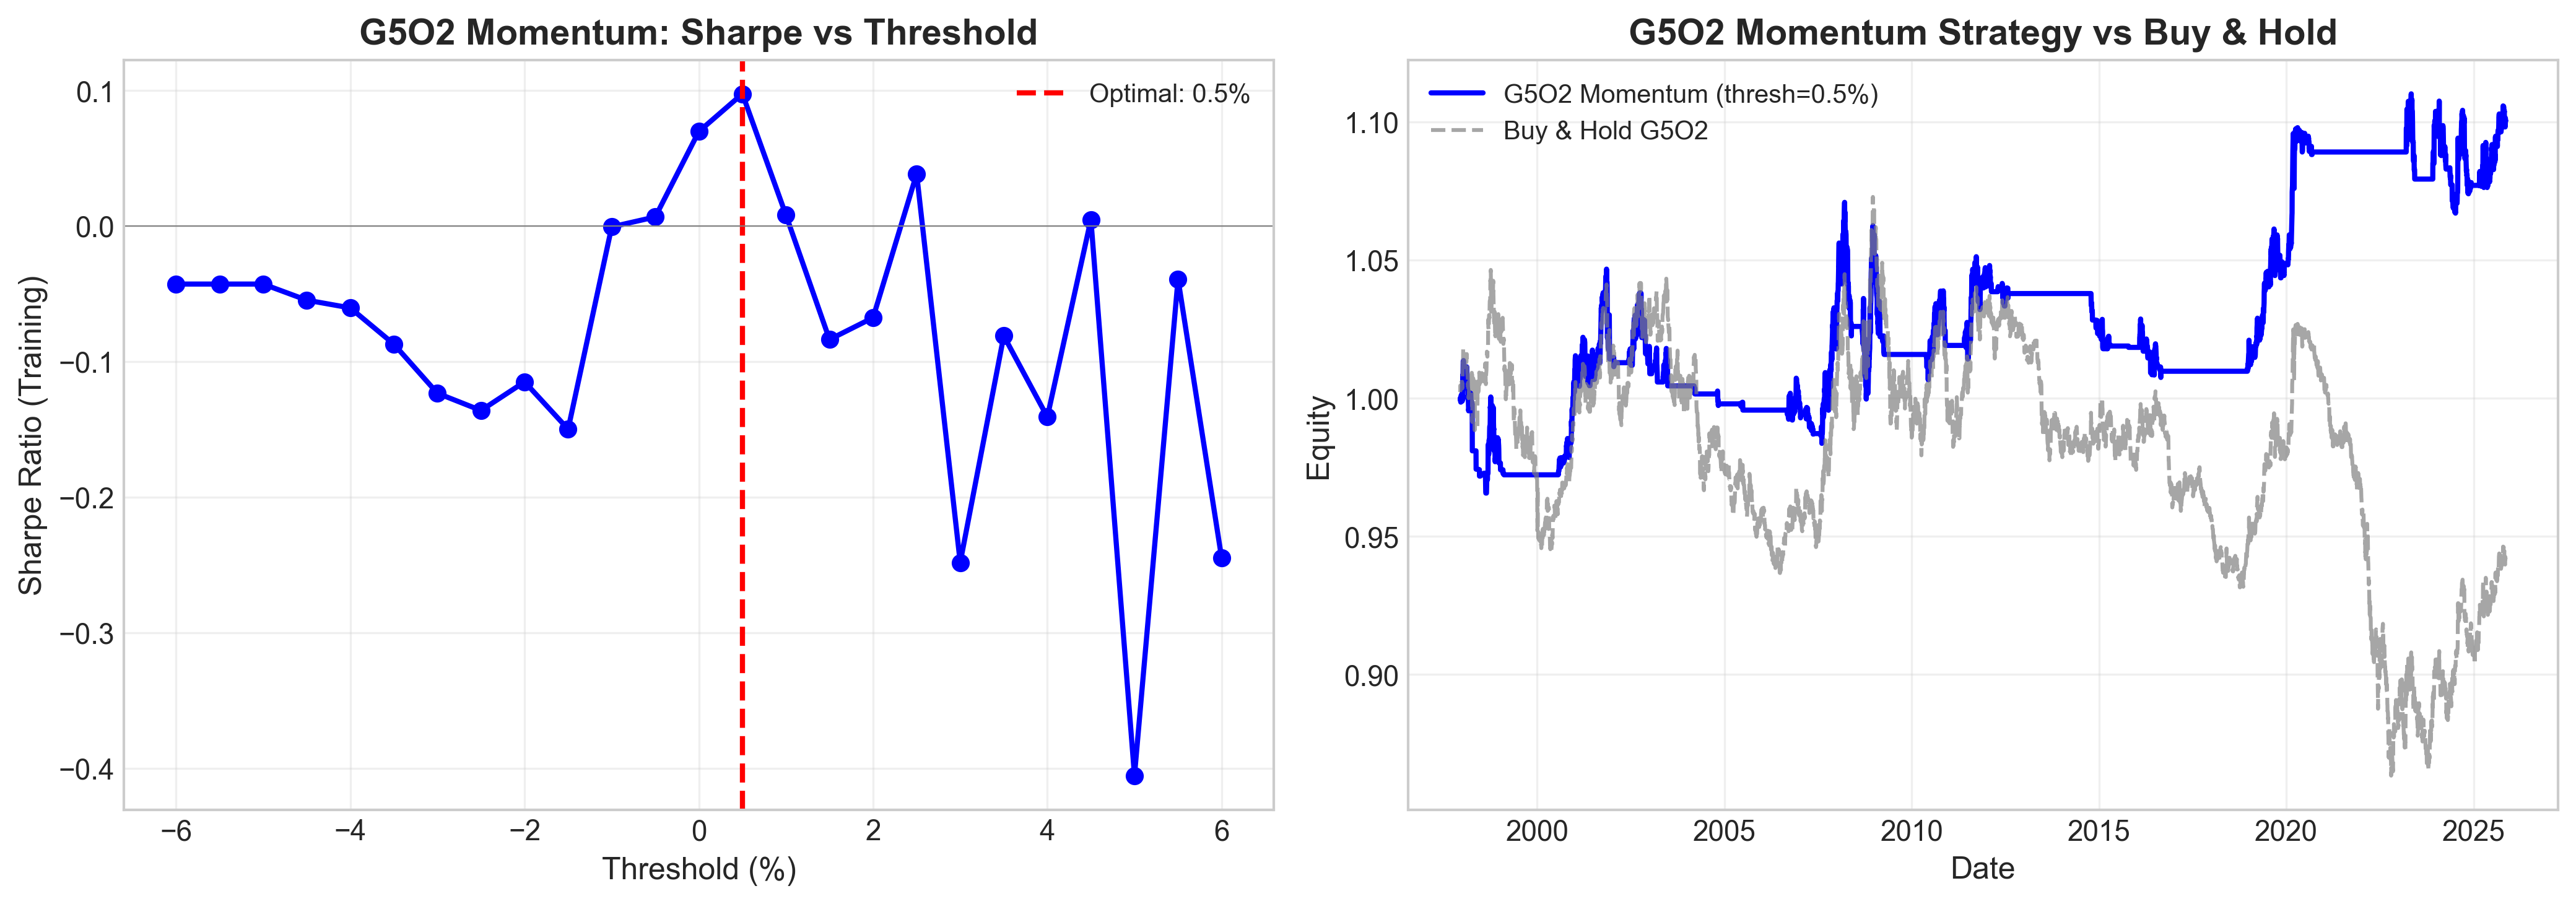
\includegraphics[width=\textwidth]{fig_g502_threshold.png}
    \caption{G5O2 momentum threshold optimization. Left panel: Sharpe ratio versus threshold across training period; optimal threshold at 0.5\%. Right panel: Momentum strategy equity curve versus buy-and-hold G5O2.}
    \label{fig:g502_threshold}
\end{figure}

The standalone G5O2 momentum strategy achieves a Sharpe ratio of 0.161, annualized return of 0.34\%, volatility of 2.13\%, maximum drawdown of $-6.65\%$, and time in market of 34.8\%. By reducing G5O2 exposure to confirmed uptrends only, the momentum variants improve overall portfolio Sharpe from 0.36/0.26 to 0.37/0.37.

\subsection{Proportional Linear Allocation}

Portfolio construction uses a proportional linear allocation mechanism that translates signal strength into position sizing. For each asset $i$ with an active signal:

\begin{equation}
\text{Score}_i(t) = \max(0, \text{BMOM}_i(t)) \times \text{Signal}_i(t)
\end{equation}

\begin{equation}
w_i^{\text{raw}} = \frac{\text{Score}_i}{\sum_j \text{Score}_j} \times 0.95
\end{equation}

with 5\% held as a liquidity buffer. The framework then applies sequential constraint enforcement:

\begin{enumerate}
    \item \textbf{Defensive mode}: If all scores equal zero, allocate 10\% cash and 90\% G5O2 (flight-to-quality positioning)

    \item \textbf{Minimum position floor}: 5\% per active asset (prevents trivially small allocations that incur transaction costs without meaningful portfolio impact)

    \item \textbf{High yield cap}: H5A4 $\leq$ 12\% per Regentfund guidelines; excess redistributed to C5A0, then G5O2, then cash
\end{enumerate}

Proportional allocation is appropriate for fixed income because momentum signal strength corresponds to the degree of trend persistence in underlying credit or rate factors. A stronger BMOM signal for investment grade credit implies more sustained spread tightening---a fundamental, not statistical, signal that justifies larger position sizing.

% =============================================================================
% SECTION 3: THE FOUR FINAL STRATEGIES
% =============================================================================
\section{The Four Final Strategies}

These four strategies represent the full implementation space defined by two binary choices: the G5O2 signal type (standard cross-asset vs. momentum-threshold) and the rebalancing cadence (daily with turnover filter vs. monthly with risk override).

\subsection{Strat 3 --- Daily Proportional Allocation}

Strat 3 is the research-optimal strategy: it runs the proportional linear allocation engine daily, applying a 5\% turnover filter to suppress unnecessary rebalancing. If the maximum weight change across all assets is less than 5 percentage points, no trade is executed. It uses the Strategy 2 drawdown-differential signal for H5A4 and C5A0, and the Strategy 2 signal for G5O2.

\begin{table}[H]
\centering
\caption{Strat 3 Performance Metrics}
\begin{tabular}{lr}
\toprule
\textbf{Metric} & \textbf{Value} \\
\midrule
Annualized Return & 1.07\% \\
Annualized Volatility & 2.95\% \\
Sharpe Ratio & 0.36 \\
Maximum Drawdown & $-11.71\%$ \\
Win Rate & 50.83\% \\
Trades per Month & 2.79 \\
\bottomrule
\end{tabular}
\end{table}

\begin{figure}[H]
    \centering
    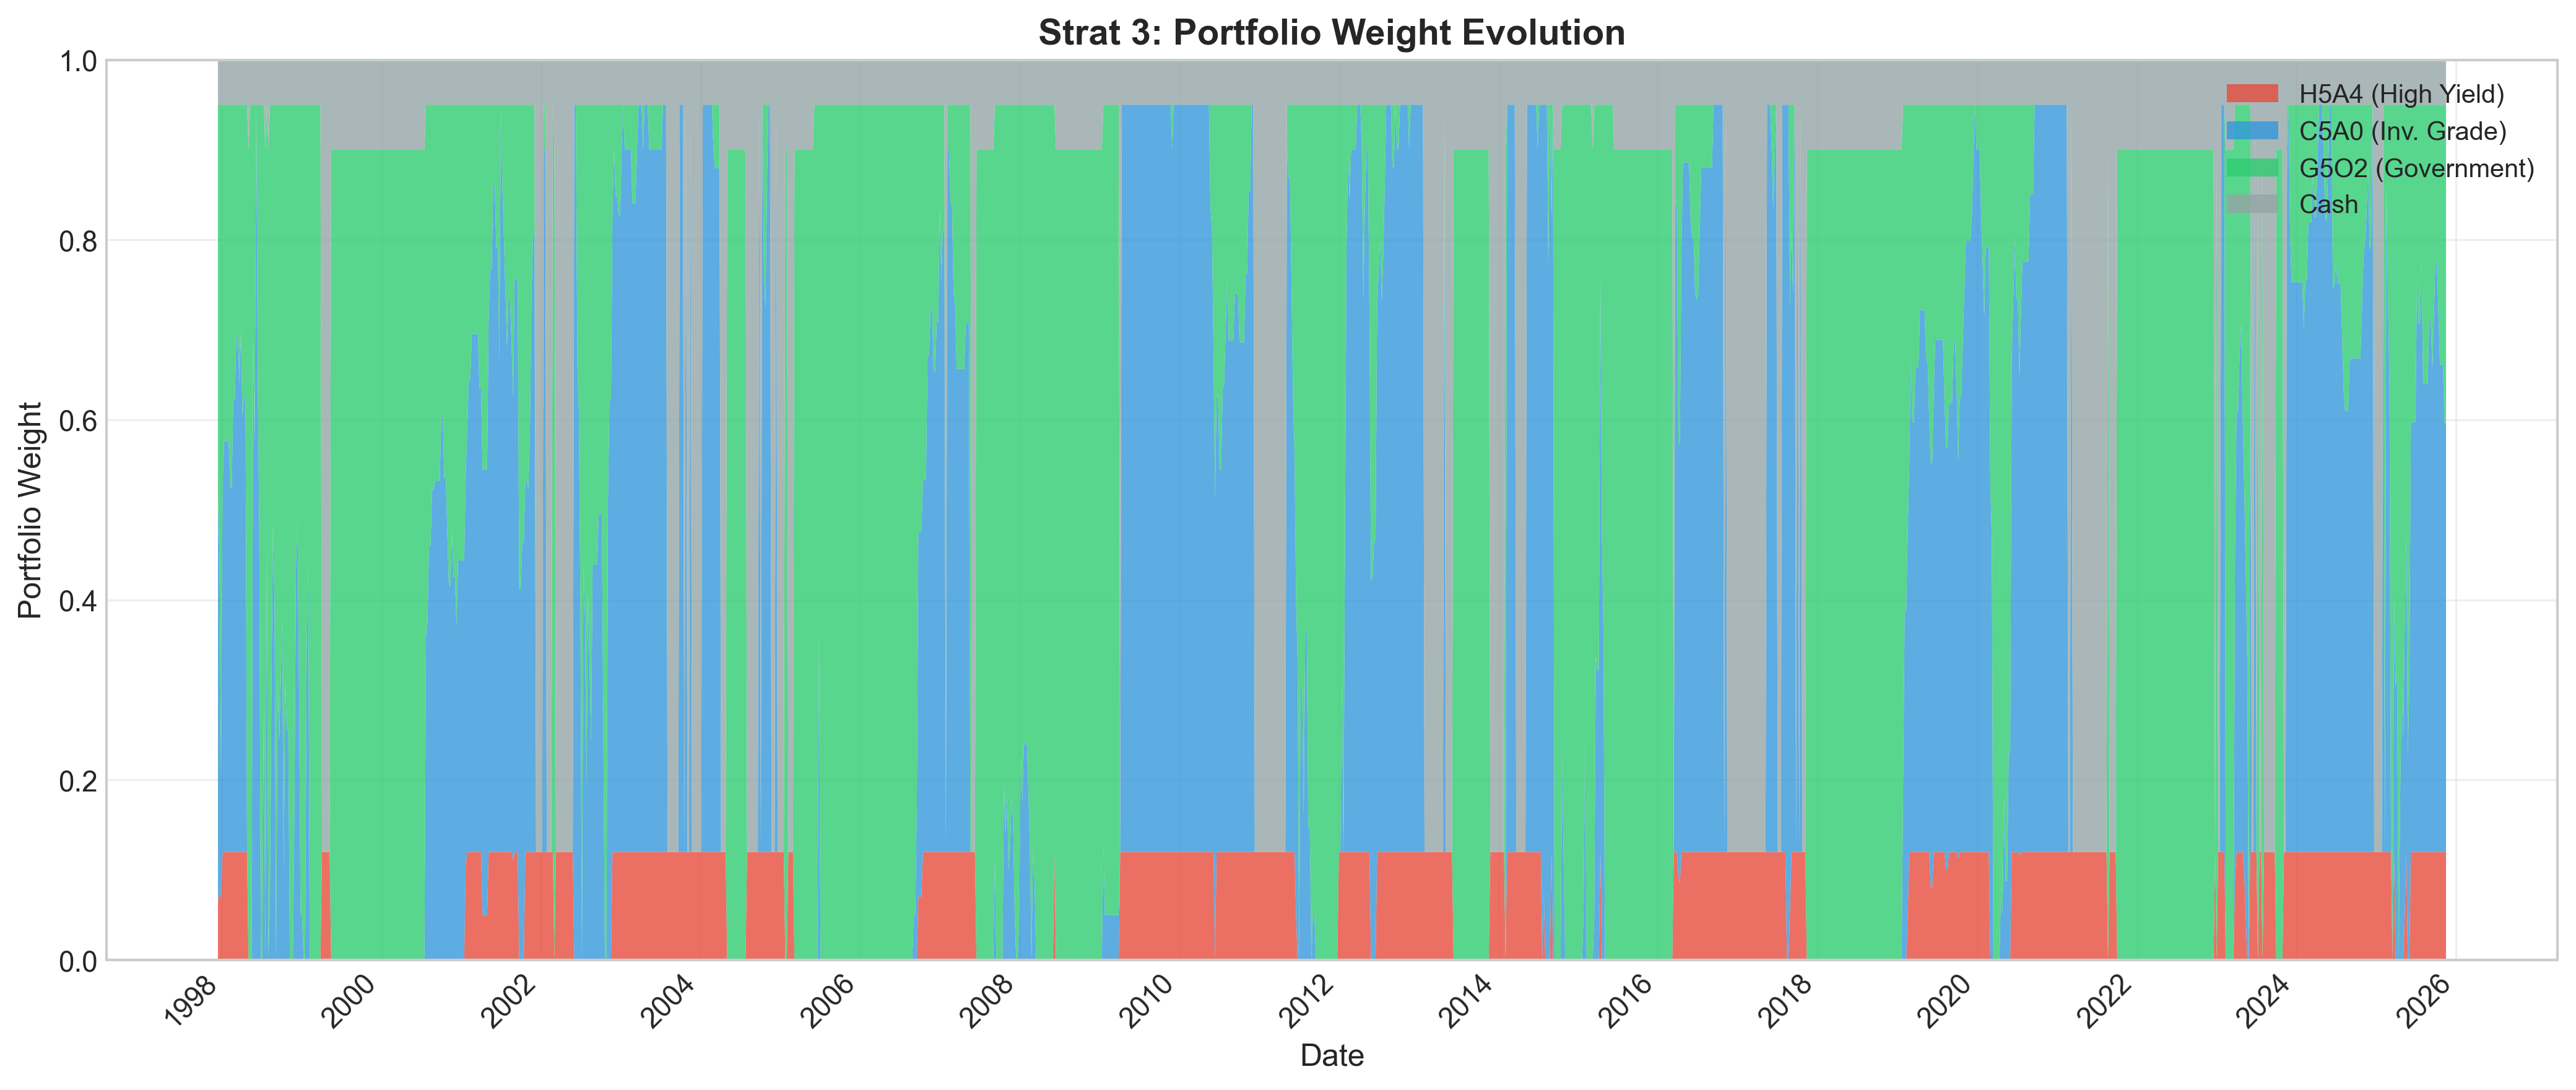
\includegraphics[width=\textwidth]{fig_strat3_weights.png}
    \caption{Strat 3 portfolio weight evolution. Note defensive rotations to high G5O2 allocation during credit stress events (2008, 2020) and active periods with maximum H5A4 exposure capped at 12\%.}
    \label{fig:strat3_weights}
\end{figure}

Figure~\ref{fig:strat3_weights} illustrates how Strat 3's weight evolution reflects fixed income regime dynamics. Periods of defensive rotation (high G5O2, low/zero HY) correspond to credit stress events, while risk-on periods feature maximum permitted H5A4 exposure and heavy investment grade allocation during spread compression.

\subsection{Monthly Strat --- Institutionally Constrained Implementation}

The Monthly Strategy adapts Strat 3 to Regentfund's monthly trading schedule via a dual-trigger approach:

\begin{itemize}
    \item \textbf{Scheduled rebalancing}: Weights are recalculated at each month-end using the proportional linear engine

    \item \textbf{Risk-triggered override}: If any asset's Strategy 2 signal turns to flat (0) intramonth, weights are immediately rebalanced without waiting for month-end
\end{itemize}

\begin{table}[H]
\centering
\caption{Monthly Strategy Performance Metrics}
\begin{tabular}{lr}
\toprule
\textbf{Metric} & \textbf{Value} \\
\midrule
Annualized Return & 0.77\% \\
Annualized Volatility & 2.97\% \\
Sharpe Ratio & 0.26 \\
Maximum Drawdown & $-11.99\%$ \\
Win Rate & 51.05\% \\
Trades per Month & 1.79 \\
\bottomrule
\end{tabular}
\end{table}

The performance gap versus Strat 3 (Sharpe 0.26 vs. 0.36) reflects the inherent limitations of monthly rebalancing: the strategy can fail to capture short-lived spread compression or relief rallies that occur mid-month, and may be slightly slower to exit into defensive positioning during rapid credit deterioration. However, the near-identical win rates (51.05\% vs. 50.83\%) confirm that core signal accuracy is preserved---the monthly constraint reduces signal capture efficiency, not signal quality.

\begin{figure}[H]
    \centering
    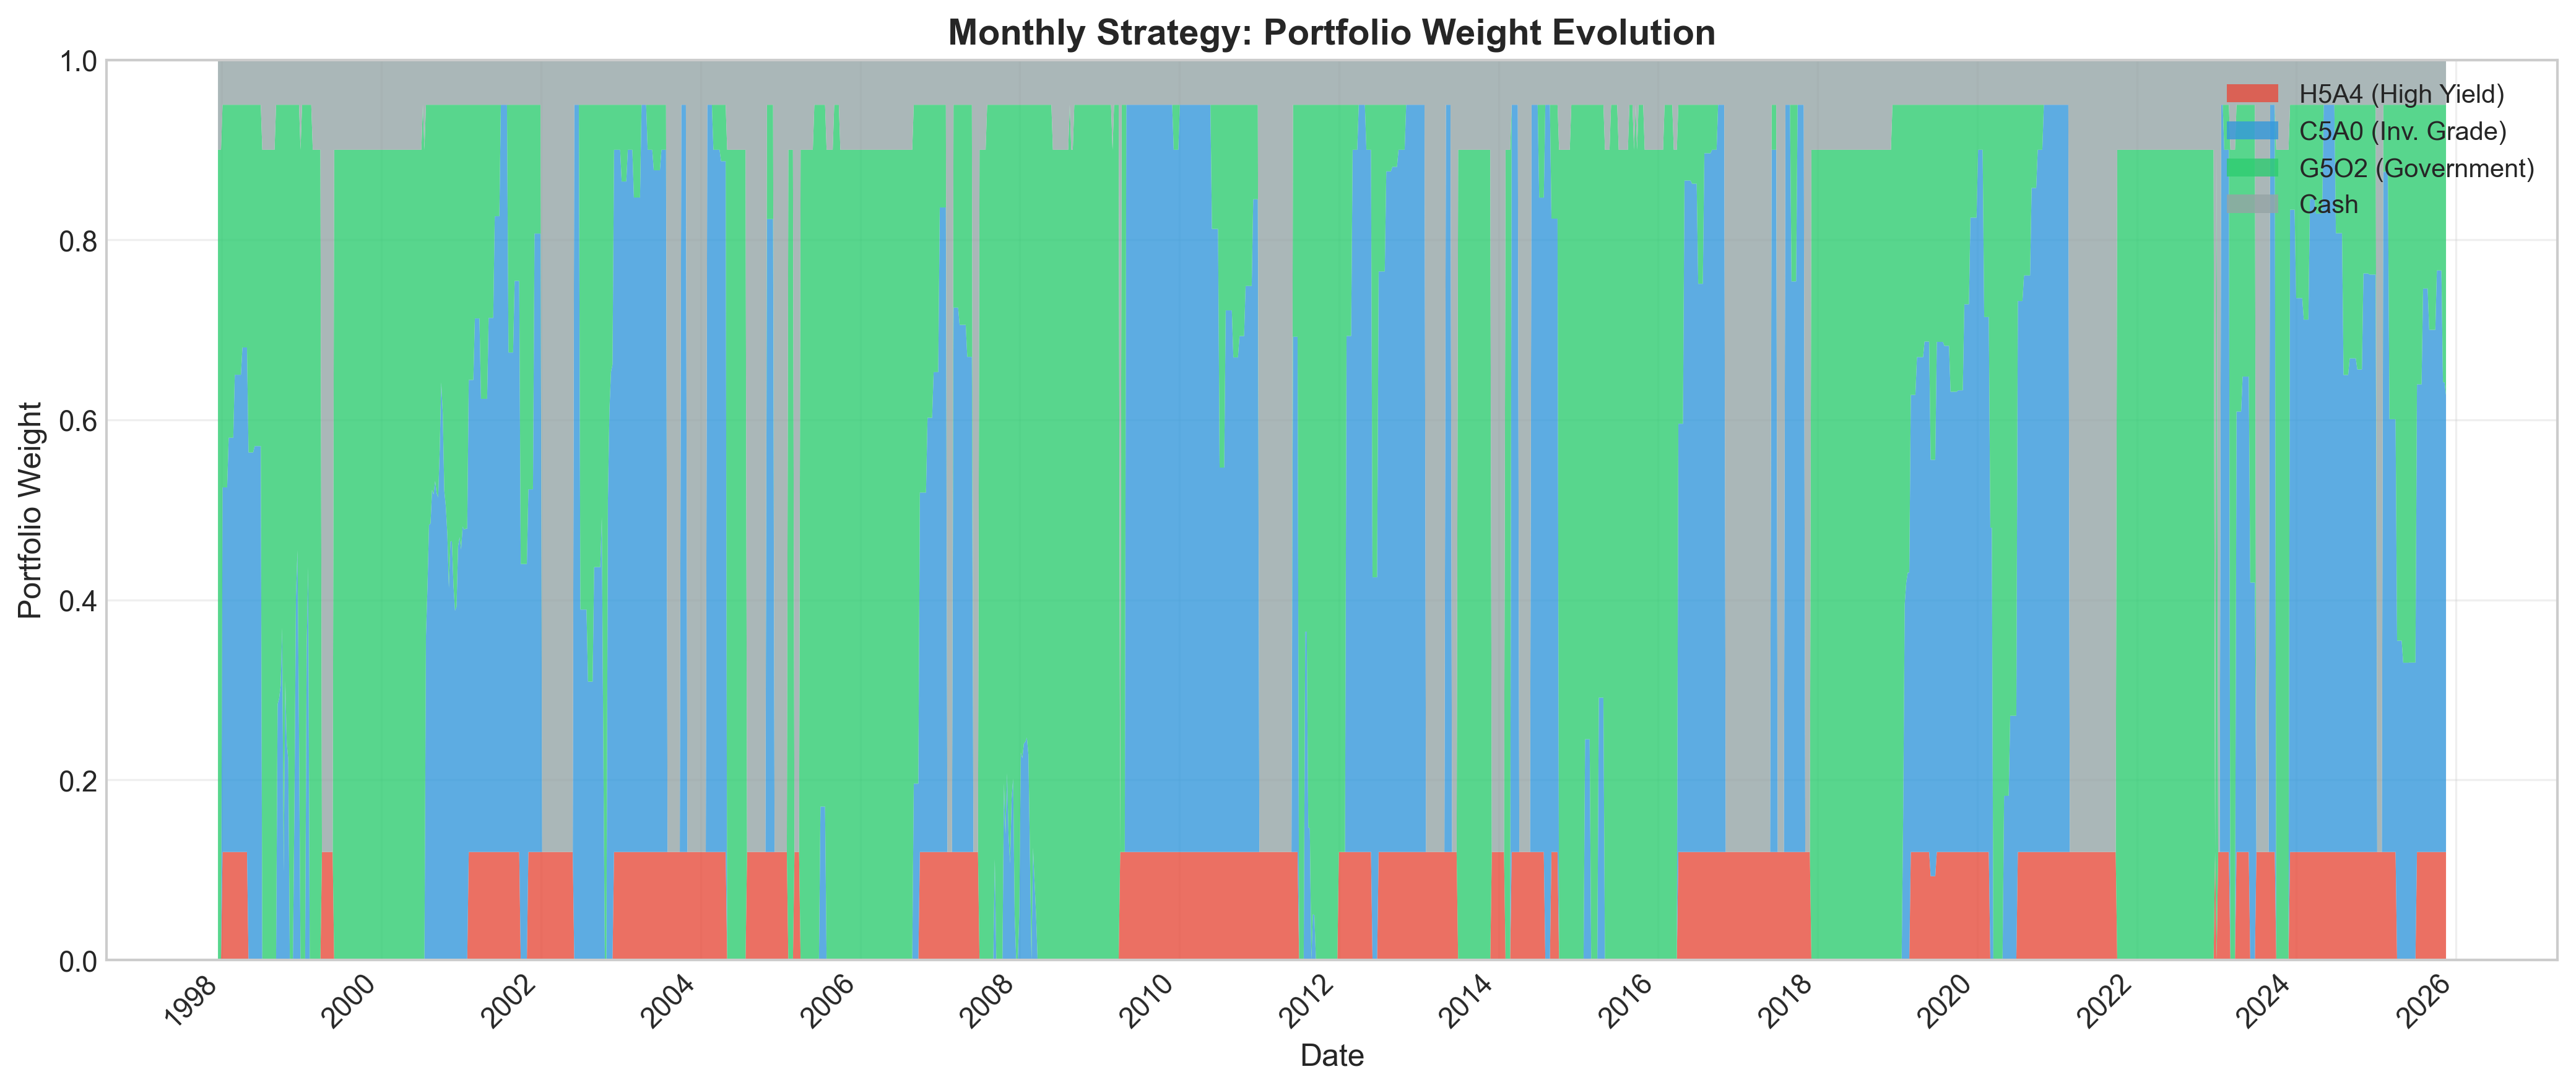
\includegraphics[width=\textwidth]{fig_monthly_weights.png}
    \caption{Monthly Strategy portfolio weight evolution. Note the characteristic step-function pattern of periodic rebalancing compared to Strat 3's more frequent adjustments.}
    \label{fig:monthly_weights}
\end{figure}

\subsection{Strat 3 (Momentum) --- Refined G5O2 Signal}

Identical to Strat 3 but replaces the Strategy 2 drawdown-differential signal for G5O2 with the standalone momentum-threshold signal (long G5O2 only when $\text{BMOM}_{\text{G5O2}} > 0.50\%$). This is the recommended implementation for Regentfund.

\begin{table}[H]
\centering
\caption{Strat 3 (Momentum) Performance Metrics}
\begin{tabular}{lr}
\toprule
\textbf{Metric} & \textbf{Value} \\
\midrule
Annualized Return & 1.09\% \\
Annualized Volatility & 2.95\% \\
Sharpe Ratio & 0.37 \\
Maximum Drawdown & $-11.71\%$ \\
Win Rate & 50.93\% \\
Trades per Month & 2.60 \\
\bottomrule
\end{tabular}
\end{table}

The improvement reflects that Treasuries are fundamentally different from credit assets. The cross-asset SPY benchmark filter is conceptually misaligned for duration assets---Treasury prices often rise when equities fall, making the dual-weakness criterion rarely and noisily triggered for G5O2. A direct momentum threshold on G5O2's own BMOM is both theoretically cleaner and empirically superior.

\subsection{Monthly Strat (Momentum) --- Recommended Implementation}

Combines the monthly rebalancing framework with the refined G5O2 momentum signal.

\begin{table}[H]
\centering
\caption{Monthly Strategy (Momentum) Performance Metrics}
\begin{tabular}{lr}
\toprule
\textbf{Metric} & \textbf{Value} \\
\midrule
Annualized Return & 1.09\% \\
Annualized Volatility & 2.97\% \\
Sharpe Ratio & 0.37 \\
Maximum Drawdown & $-11.71\%$ \\
Win Rate & 50.99\% \\
Trades per Month & 4.70 \\
\bottomrule
\end{tabular}
\end{table}

The higher trades per month (4.70 vs. 1.79 for Monthly Strat) reflects more frequent G5O2 signal transitions from the momentum-threshold approach, which is more active in G5O2 than the drawdown-differential approach. Importantly, despite higher trading frequency, performance is superior---these trades are signal-driven, not noise-driven.

% =============================================================================
% SECTION 4: RESULTS AND PERFORMANCE ANALYSIS
% =============================================================================
\section{Results and Performance Analysis}

\subsection{Comparison to Benchmark}

The static benchmark delivered $-0.14\%$ annualized return with $-20.89\%$ maximum drawdown and a Sharpe ratio of $-0.04$ over the full sample period. All four tactical strategies outperform on every risk-adjusted metric.

\begin{table}[H]
\centering
\caption{Complete Performance Comparison}
\label{tab:full_comparison}
\begin{tabular}{lcccccc}
\toprule
\textbf{Strategy} & \textbf{Ann. Ret.} & \textbf{Ann. Vol.} & \textbf{Sharpe} & \textbf{Max DD} & \textbf{Win Rate} & \textbf{Trades/Mo} \\
\midrule
Strat 3 & 1.07\% & 2.95\% & 0.36 & $-11.71\%$ & 50.83\% & 2.79 \\
Monthly Strat & 0.77\% & 2.97\% & 0.26 & $-11.99\%$ & 51.05\% & 1.79 \\
Strat 3 (Momentum) & 1.09\% & 2.95\% & 0.37 & $-11.71\%$ & 50.93\% & 2.60 \\
Monthly (Momentum) & 1.09\% & 2.97\% & 0.37 & $-11.71\%$ & 50.99\% & 4.70 \\
\midrule
Benchmark (B\&H) & $-0.14\%$ & 3.35\% & $-0.04$ & $-20.89\%$ & 50.42\% & 0.0 \\
\bottomrule
\end{tabular}
\end{table}

The benchmark's underperformance is not surprising given the sample period (1997--2025) includes three major credit stress events and a sustained rising rate environment. A static allocation is structurally exposed to all of these simultaneously, with no mechanism to reduce high yield exposure when credit spreads blow out or reduce investment grade duration when rates rise sharply.

\textbf{The tactical framework's 43\% reduction in maximum drawdown---from $-20.89\%$ to approximately $-12\%$---represents the single most practically important result for an institutional fixed income portfolio.} Capital preservation during crisis periods is the primary mandate for fixed income allocations; the strategies deliver this protection while generating positive risk-adjusted returns.

\subsection{Equity Curve Analysis}

\begin{figure}[H]
    \centering
    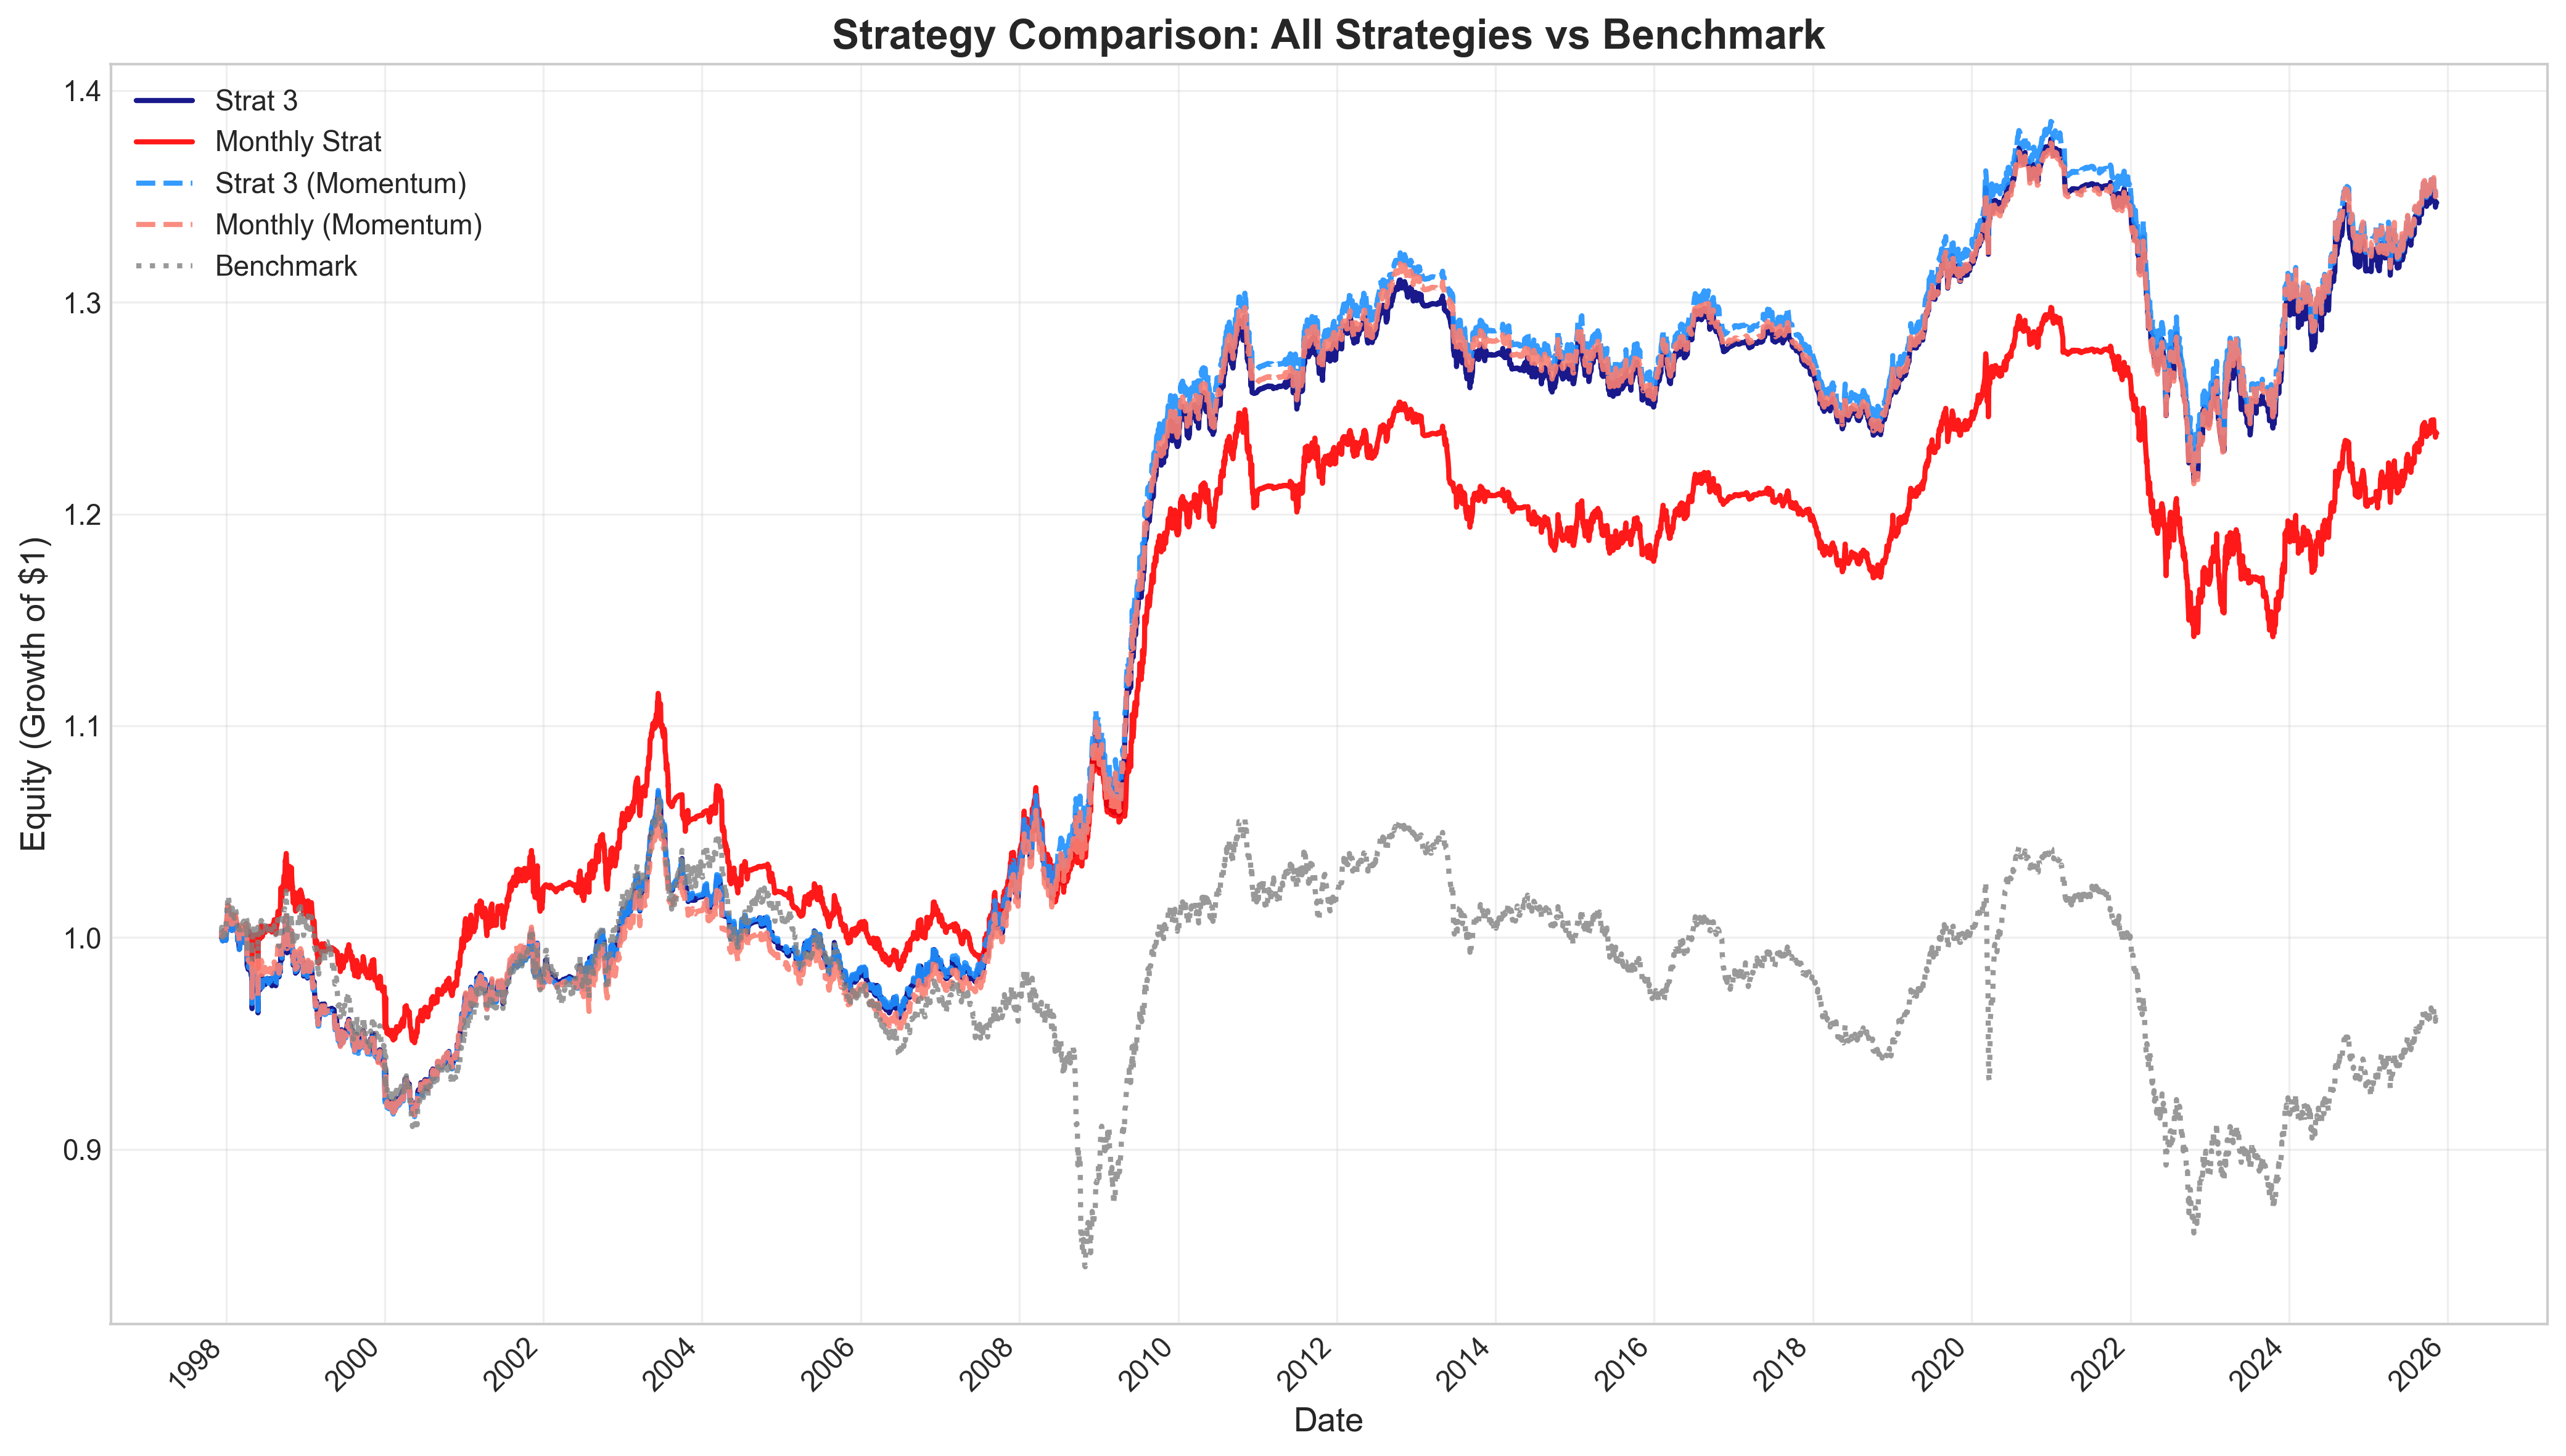
\includegraphics[width=\textwidth]{fig_strategy_comparison.png}
    \caption{Equity curve comparison: all four strategies versus benchmark. The divergence from benchmark begins clearly around 2008, confirming the crisis-avoidance mechanism.}
    \label{fig:equity_curves}
\end{figure}

Figure~\ref{fig:equity_curves} reveals several important patterns:

\begin{itemize}
    \item The divergence from benchmark begins clearly around 2008, confirming the crisis-avoidance mechanism operates during major credit events

    \item Strat 3 and its Momentum variant trace similar paths with marginally superior terminal wealth

    \item Monthly strategies show the characteristic step-function of periodic rebalancing but maintain the key property of avoiding the benchmark's prolonged drawdowns

    \item The post-2022 period is notable: while the benchmark partially recovered, it never fully recovered the 2021--2022 rate-shock losses; the tactical strategies' defensive repositioning during rate deterioration preserved substantially more capital
\end{itemize}

\subsection{Drawdown Analysis}

\begin{figure}[H]
    \centering
    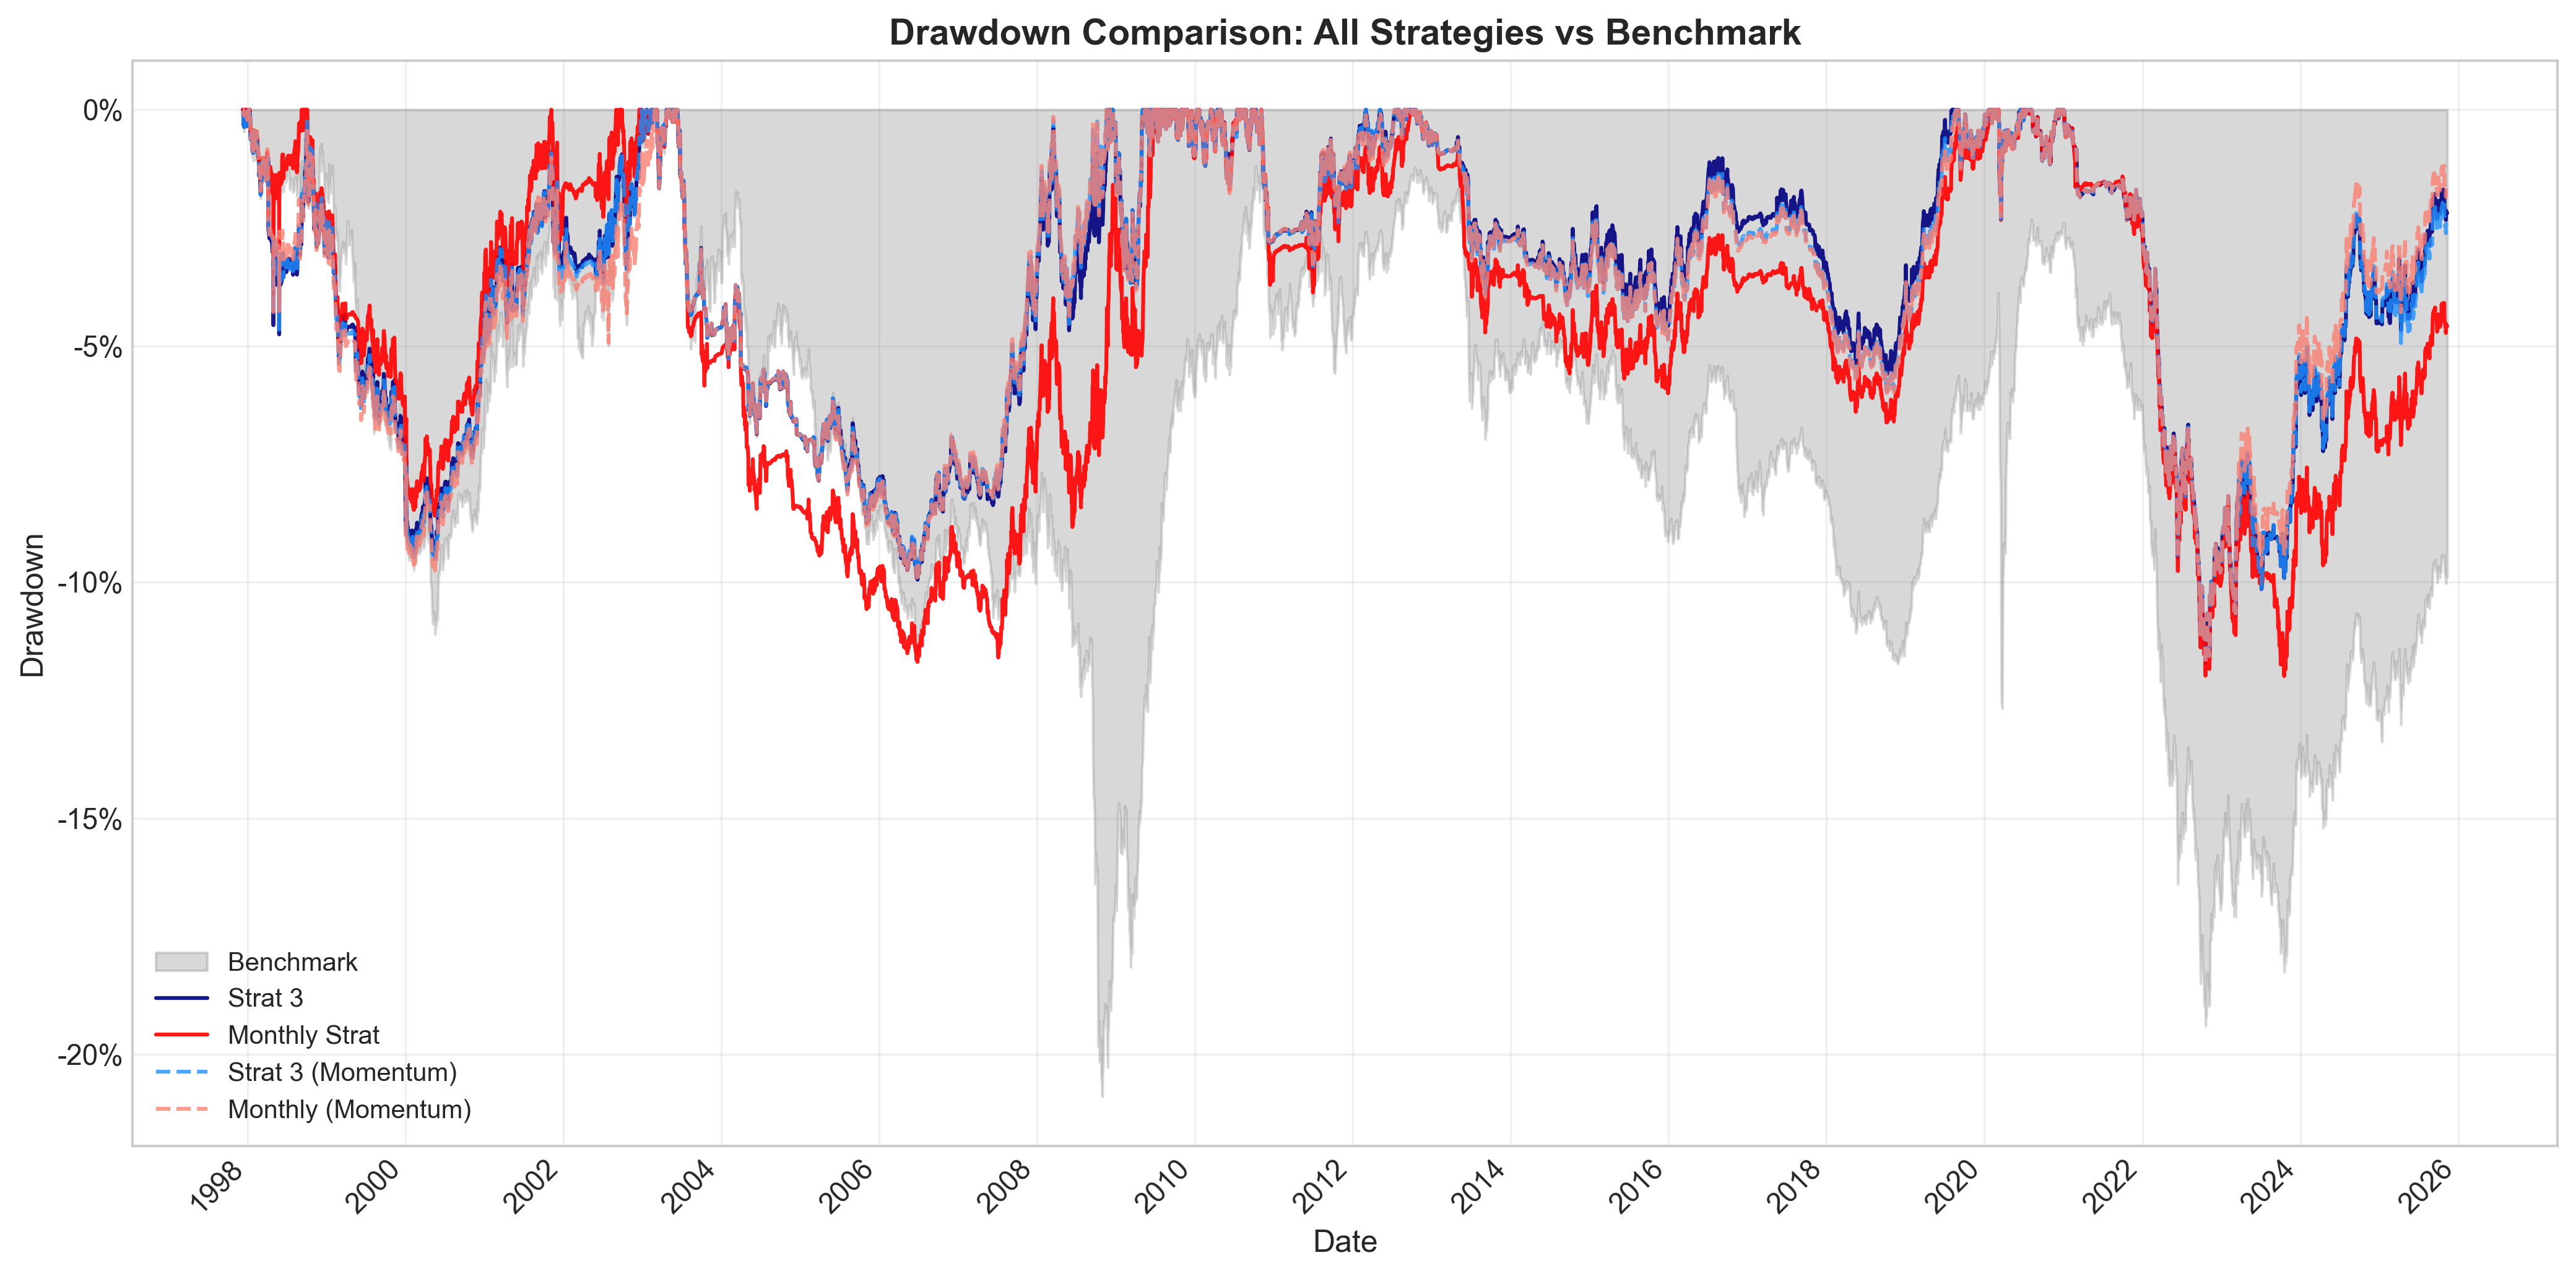
\includegraphics[width=\textwidth]{fig_drawdown_comparison.png}
    \caption{Drawdown comparison across all strategies. The benchmark (grey fill) experiences three major drawdown periods exceeding 15\%; all tactical strategies substantially reduce these events.}
    \label{fig:drawdowns}
\end{figure}

For a fixed income audience, drawdown analysis is arguably more important than return analysis---institutional mandates often have explicit drawdown limits, and fixed income is frequently selected precisely for its capital preservation characteristics.

Figure~\ref{fig:drawdowns} highlights:
\begin{itemize}
    \item The benchmark's three major drawdown periods corresponding to the 2001--02 credit cycle, 2008 financial crisis, and 2022 rate shock

    \item All four strategies avoided or substantially reduced each of these drawdowns

    \item The $-11.71\%$ to $-11.99\%$ max drawdown range across strategies reflects a structural floor driven by the lag between signal generation and execution, not a model failure
\end{itemize}

\subsection{Strategy Selection Guidance}

\begin{itemize}
    \item \textbf{Recommended: Strat 3 (Momentum)}---highest Sharpe (0.37), lowest drawdown ($-11.71\%$), fewest trades among momentum variants (2.60/month), cleanest duration logic with conceptually appropriate G5O2 signal

    \item \textbf{If monthly rebalancing is required (institutional constraint)}: Monthly Strat (Momentum)---matches monthly operational requirements while achieving the same Sharpe as daily strategies

    \item \textbf{If operational simplicity is paramount over maximum performance}: Monthly Strat (Standard)---fewest trades per month (1.79), simplest signal for G5O2, modest but meaningful outperformance vs. benchmark
\end{itemize}

% =============================================================================
% SECTION 5: RISK CONSIDERATIONS AND LIMITATIONS
% =============================================================================
\section{Risk Considerations and Limitations}

\subsection{Signal Lag Risk}

The cross-below detection mechanism requires momentum to already be deteriorating before signals exit. In sharp, rapid credit selloffs (e.g., March 2020), the strategy may absorb initial losses before the signal triggers an exit. The $-12\%$ maximum drawdown reflects this structural lag between market deterioration and defensive repositioning.

\subsection{Rebalancing Frequency Risk}

Monthly rebalancing creates intramonth exposure drift. Between rebalance dates, portfolio weights drift with market movements and cannot be corrected until the next scheduled date (except via the risk-triggered override). In volatile credit markets, this can result in unintended concentration or de-risking timing that deviates from optimal positioning.

\subsection{G5O2 Momentum Threshold Stability}

The 0.5\% optimal threshold for G5O2 momentum signal was identified via in-sample training (1997--2014) and tested out-of-sample (2014--2025). Signal thresholds in momentum strategies can be regime-sensitive; the threshold should be reviewed periodically as rate environments shift structurally. Significant changes in Federal Reserve policy frameworks or Treasury market microstructure could alter the optimal threshold.

\subsection{Parameter Sensitivity}

The drawdown differential override threshold (10 percentage points) and BMOM weights (0.15/0.35/0.35/0.15) were developed through iterative research grounded in economic reasoning about credit and rate cycle frequencies. While theoretically motivated, parameter sensitivity analysis should be conducted before live deployment to ensure robustness to reasonable perturbations.

\subsection{Transaction Costs}

All performance metrics are gross of transaction costs. In practice, the 1.79--4.70 trades per month across strategies with typical bid-ask spreads in investment grade and government bond markets represents a modest but non-negligible implementation cost. Net Sharpe ratios will be somewhat lower than reported figures; the magnitude depends on execution quality and portfolio scale.

% =============================================================================
% SECTION 6: CONCLUSION
% =============================================================================
\section{Conclusion}

This paper presents a systematic tactical allocation framework for fixed income portfolios that addresses the fundamental challenge of time-varying risk premia in credit and duration markets. The key insight is that credit and duration momentum are not behavioral anomalies to be arbitraged---they are systematic reflections of the slow-moving, fundamental nature of fixed income risk factor dynamics.

Credit cycles turn gradually as corporate fundamentals evolve; spreads widen progressively as lenders reassess default probabilities, covenant violations accumulate, and rating agencies downgrade issuers. Rate regimes persist as central bank policy adjusts to macroeconomic conditions on multi-quarter horizons. The BMOM framework captures these dynamics at the appropriate time horizons, while the cross-asset filter leverages the equity market's superior liquidity and information efficiency as an early warning system.

Strat 3 (Momentum) is the recommended implementation for Regentfund: it delivers a 0.37 Sharpe ratio with a $-11.71\%$ maximum drawdown versus the benchmark's $-0.04$ Sharpe and $-20.89\%$ maximum drawdown, while adhering to the 12\% high yield cap and achieving the highest risk-adjusted returns among all variants.

The framework's value proposition for institutional fixed income portfolios is clear: systematic, rules-based risk management that delivers capital preservation during crisis periods while capturing positive risk-adjusted returns during normal market conditions. Future enhancements could include LASSO-based feature selection across a broader momentum horizon set and regime classification methodologies to improve the identification of credit stress versus rate stress environments.

% =============================================================================
% END DOCUMENT
% =============================================================================
\end{document}
